

%\renewcommand\thesection{\Alph{section}}
%\section[Improper priors]{Improper priors} 
%\titleformat{\chapter}
\chapter*{Appendix A}\label{AppendixA}

\vspace{-1.75cm}
\subsection*{Improper priors}

The penalty matrix $\mathbf{P}$ corresponding to an undirected $RW_\kappa$ prior over 
parameter vector $\lambda \in \mathbb{R}^C$ has rank $C - \kappa$ and the resulting 
matrix $\Sigma^{-1} = \mathbf{Q} = \mathbf{P}/\tau^2$ is singular and thus not a valid precision 
matrix. In the $RW_1$ case this can be mitigated by jittering the elements of $\mathbf{P}$. 
For $\kappa > 1$ a possibility is to estimate only $C - \kappa$ of the $C$ parameters in $\lambda$,  
from which the remaining $\kappa$ so-called {\it pinned} parameters (each of which has a 
conditional variance of zero) can be computed following the properties of the multivariate 
normal distribution. This strategy amounts to  constraining the relevant linear combinations 
to have zero variance, from which a proper prior on a lower dimensional subspace is 
obtained \shortcite{paciorek_2009, rue_gaussian_2005}. 

Another possibility is to estimate the autoregressive parameter $\omega$ mentioned 
in \ref{penalty_matrix} (see footnote~\ref{footnote_car}), which results in a proper prior.
\citeA<See>{paciorek_2009} \citeA<and>{banerjee_hierarchical_2004} for potential
drawbacks to this approach.

An entirely different tactic would be to estimate an arbitrary tridiagonal precision matrix 
rather than specifying the penalty matrix and estimating the hierarchical variance/precision 
parameter. One way to do this would be to decompose the precision matrix into conditional 
correlations and standard deviations. This is possible to do in Stan and should be explored 
in future work to sidestep the matrix singularity problems. 


\chapter*{Appendix B}\label{AppendixB}
\vspace{-1.75cm}

\subsection*{Seats-votes curves}

Seats-votes curves for various values of $\lambda$ (bias) and $\rho$ (responsiveness). 
In the first plot $\lambda$ is fixed at 0 and the value of $\rho$ varies. In the second plot 
$\rho$ is fixed at 1 and the value of $\lambda$ varies. 

\begin{figure}[h]
\centering
	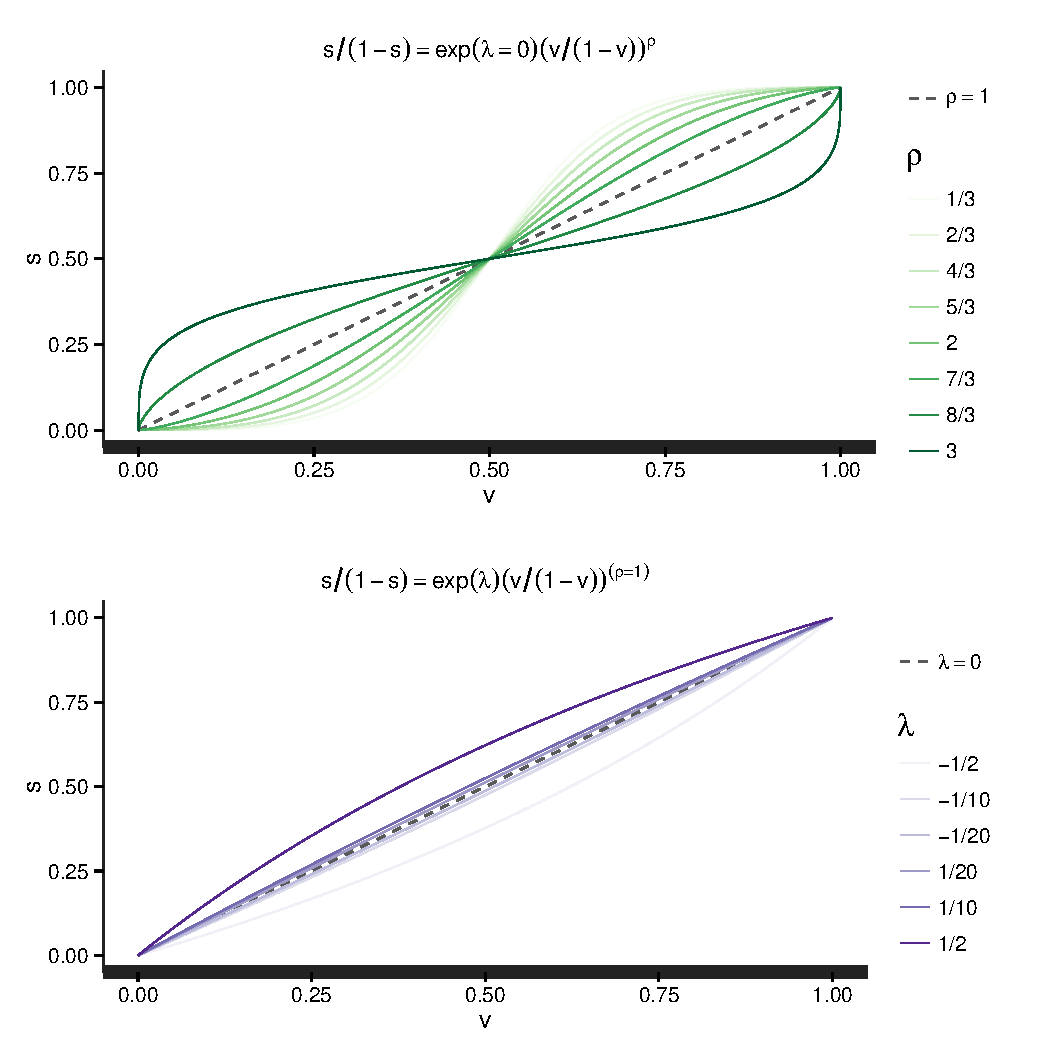
\includegraphics[scale=0.8]{sections/figs/seats_votes}
\label{fig:seats_votes}
\end{figure}


\chapter*{Appendix C}\label{AppendixC}
\vspace{-1.75cm}
\subsection*{Parameter estimates}

Estimates (on the logit scale) of $\lambda$ and $\rho$ from the Bayesian STAR model. 
The darker ribbons show 50\% posterior intervals and the lighter ribbons are 95\% 
intervals. The connected points are posterior medians. 
(Note that the $y$-axis is scaled differently for each parameter.) 

\vspace{.5cm}

\begin{figure}[h]
\centering
	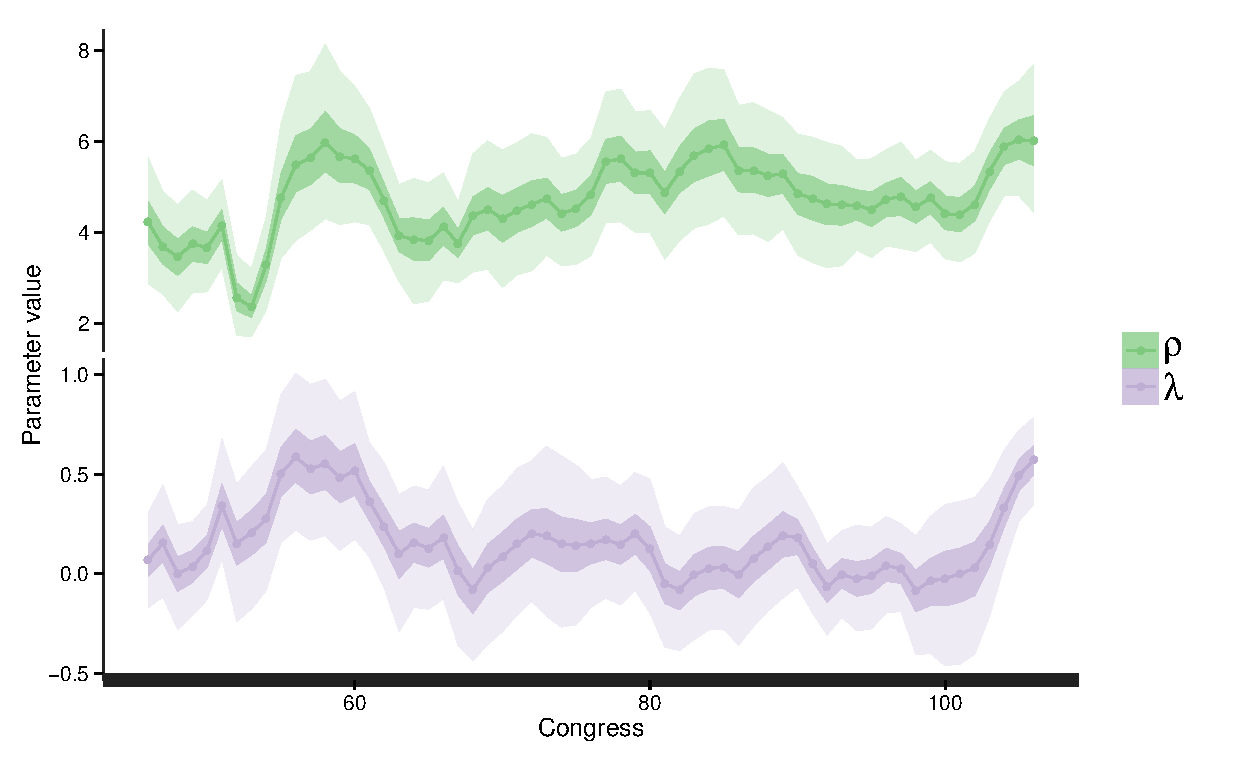
\includegraphics[scale=0.8]{sections/figs/lambda_rho}
\label{fig:lambda_rho}
\end{figure}





\chapter*{Appendix D}\label{AppendixD}
\vspace{-1.75cm}
\subsection*{Hamiltonian Monte Carlo}

The following is a simplified version of the HMC algorithm employed by Stan. 

{\singlespacing
\subsubsection{Notation}

\begin{tabular}{ll}
$\theta$ & D-dimensional position vector (model parameters to be estimated) \\

 $ \rho$ & D-dimensional vector of auxiliary momentum variables \\

$\mathcal{L}$ & Natural logarithm of joint probability density for $\theta$ (up to normalizing constant) \\

$\nabla_\theta$ & Gradient with respect to $\theta$ \\

$x^{[t]}$ & Value of $x$ at time $t$ \\

$N$ & Number of iterations to run the algorithm \\

$L$ & Number of ``leapfrog" steps (to run the simulated Hamiltonian system) per iteration\\

$\epsilon$ & Size of the leapfrog steps
\end{tabular}
}
\vskip.5cm

\subsubsection{Leapfrog function}

A single leapfrog update consists of executing the following function once:

{\singlespacing

${\tt leapfrog} (\rho, \theta, \epsilon) \{$ 

\begin{tabular}{ll}
$\quad \tilde{\rho} \leftarrow \rho + \tfrac{1}{2}\epsilon \nabla_\theta \mathcal{L}(\theta)$ & {\it (half step)} \\

$\quad \tilde{\theta} \leftarrow \theta + \epsilon \tilde{\rho}$ & {\it (full step)} \\

$\quad \tilde{\rho} \leftarrow \tilde{\rho} + \tfrac{1}{2}\epsilon \nabla_\theta \mathcal{L}(\tilde{\theta})$ & {\it (half step)} \\

$\quad {\tt return} (\tilde{\rho}, \tilde{\theta})$
\end{tabular}

$\}$

}

\subsubsection{Pseudo-code for HMC algorithm}


\noindent Set $N$, $\theta^{[0]}$, $\epsilon$, and $L$.

\noindent For $n = 1, \dots, N \quad \{$ 

\begin{tabular}{ll}
{\bf (i)} $\rho^{[0]} \sim \mathcal{N}_D(0, \mtrx{I})$ & ({\it Sample iid standard normal inits for $\rho$}) \\

{\bf (ii)} $\tilde{\rho} \leftarrow \rho^{[0]}$, $\tilde{\theta} \leftarrow \theta^{[n-1]}$ &  ({\it Initialize $\tilde{\rho}, \tilde{\theta}$})\\

{\bf (iii)} For $\ell = 1, \dots, L \quad \{$  & ({\it Do $L$ leapfrog updates to generate proposal }) \\[-8pt]

\qquad $(\tilde{\rho}, \tilde{\theta}) \leftarrow {\tt leapfrog}(\tilde{\rho}, \tilde{\theta}, \epsilon)$ & \\[-8pt]
\quad $\}$ & \\

\quad Compute acceptance probability $p^\star$  & \\[-8pt]
$\qquad  q^{\it new} \leftarrow  \mathcal{L}(\tilde{\theta}) - \tfrac{1}{2} \tilde{\rho} \cdot \tilde{\rho} $ & \\[-8pt]
$ \qquad q^{\it old} \leftarrow   \mathcal{L}(\theta^{[n-1]} ) -  \tfrac{1}{2} \rho^{[0]} \cdot \rho^{[0]} $ & \\[-8pt]
$ \qquad p^\star = \min{\left\{1, \exp{\left( q^{\it new} - q^{\it old} \right)} \right\}} $& \\[3pt]

{\bf (iv)} Set $\theta^{[n]} \leftarrow \tilde{\theta}$ with probability $p^\star$  & ({\it Accept or reject proposal})\\
\qquad and $\theta^{[n]} \leftarrow \theta^{[n-1]}$ with probability $ 1 - p^\star$ & \\

\end{tabular}

\noindent $\}$d

Technically in {\bf (iv)} the proposal for $m$ is accepted or rejected along with the proposal for 
$\theta$, but in practice we only care about $\theta$. The momentum variables are introduced out of necessity 
in order to simulate Hamiltonian dynamics, but they are not themselves quantities of interest.

Note that the above procedure requires $\epsilon$ (step-size) and $L$ (number of steps) to be specified in 
advance. Very roughly speaking, if $L$ and/or $\epsilon$ is too small proposals for $\theta^{[n]}$ will be too 
close to $\theta^{[n-1]}$ and the chain will mix slowly, whereas if they are too large the proposals will stray 
too far and will be unlikely to be accepted. Larger values for $\epsilon$ will also lead to cruder discrete
approximations of the continuous-time Hamiltonian system. The NUTS algorithm \shortcite{hoffman_2012} 
used by Stan is designed to automatically tune $L$ and $\epsilon$ for each chain during a warmup period. 
See \citeA{hoffman_2012} for the technical details and \citeA{stan_development_team_stan_2015} for more 
on Stan's implementation. 




\chapter*{Appendix E}\label{AppendixE}
\vspace{-1.75cm}
\subsection*{Different Interpretations}

Although Figure~\ref{fig:ck_bias} (p.~\pageref{fig:ck_bias}) appears to show two versions of the same plot with
slightly different estimates, Cox and Katz's results -- obtained by maximum likelihood estimation --
and the results from the Bayesian model must be interpreted differently. The former are point estimates 
and confidence intervals, whereas the full Bayesian model provides an estimate of the marginal posterior 
{\it distribution} for each parameter. That is, the estimates obtained from the Bayesian model are the 
distributions themselves, which are representations of our uncertainty about the parameters 
given the data. 

The methods used by Cox and Katz come from the classical approach where a single point 
estimate is obtained for each parameter and assessed in relation to infinitely many intervals 
constructed from datasets obtained from hypothetical, endless repeated sampling. While in many 
situations it is natural to imagine repeating an experiment (e.g. coin flipping) or resampling from 
a population, such an interpretation is more difficult to justify in the context of the historical 
events of interest to this analysis. For each confidence interval obtained from Cox and Katz's analysis, 
what can be said is that it either contains the (theoretical) true parameter value or it does not. This is 
a consequence of accepting (explicitly or implicitly) the classical position that the parameter is fixed 
while the data and confidence interval bounds are random variables. 

On the contrary, from the Bayesian perspective the parameter is treated as a random variable while 
the data and interval bounds are fixed. As a result, any so-called credible intervals computed from the 
posterior distribution have a more intuitive interpretation: the probability that the true parameter value lies 
in the $p\%$ interval  -- conditional on the model and data -- is $p$. 



